 \chapter{Diseño del sistema} 

Para realizar el procesamiento más adecuado al sistema, en primer lugar se tendrá que entrenar con una serie de señales obtenidas de \textit{prueba} con tal fin. Una vez captadas y ajustado el algoritmo, probaremos con una batería de señales en cada brazo que este funciona como lo esperado y cumple con su objetivo. Con estos datos ya no se modificará el algoritmo de procesamiento. 

\begin{figure}[H]
	\center
	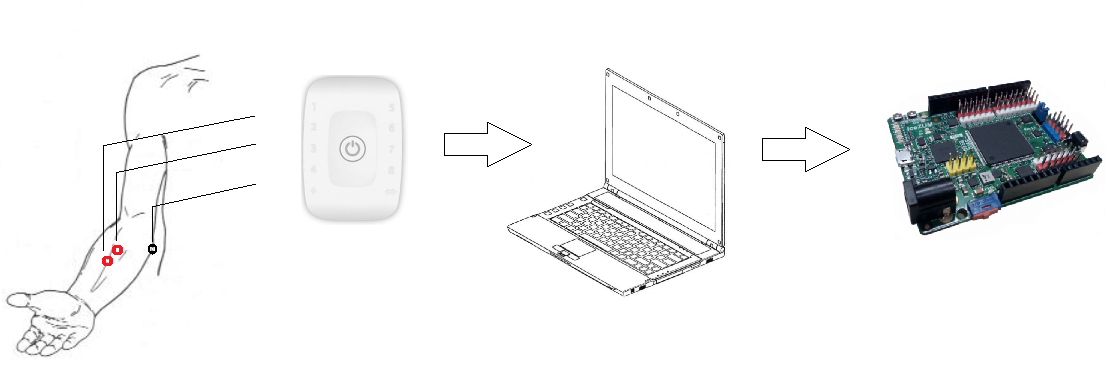
\includegraphics[scale=0.6]{imagenes/Disenodelsistema/sistema.png}
	\caption{Proceso para obtener y procesar bioseñales}
	\label{fig:Sistema}
\end{figure}


En primer lugar se captan las señales de prueba o entrenamiento, que mediante Bluethooth son enviadas al ordenador en tiempo real y recogidas en el software OpenSignals. Estas señales que hemos guardado son posteriormente procesadas en Matlab para su filtrado y captación de parámetros que nos permitan distinguir los distintos estados en los que se encuentra el músculo. El filtrado debe de ser capaz de eliminar el ruido y de acondicionar la señal para que sea más fácil distinguir sus parámetros de bondad. 
 \newline
Una vez las señales se procesan son enviadas mediante comunicación serie a la FPGA, en la que se va a definir el modo de control. Para ello se utilizará la modulación PWM, que como hemos visto en \ref{sec:comdron} es la tecnología más barata y utilizada. 

En los siguientes capítulos vamos a ver más detenidamente todo el proceso de obtención así como la implementación del proyecto.

\section{Adquisición}

En cuanto a la adquisición de señales EMG hay que tener en cuenta un correcto acondicionamiento de la piel y una colocación adecuada de los electrodos de medida.

\subsection{Preparación de la piel} \label{sec:Preparaciondelapiel}
 Es necesario a la hora de obtener señales EMG una correcta preparación de la piel dónde vamos a colocar los electrodos; de forma que la calidad de la señal obtenida sea la mejor posible. Para este propósito es recomendable usar un gel abrasivo o alcohol tanto para eliminar las células muertas de la piel como para reducir la sequedad de la misma. Tras la correcta limpieza con un paño suave se asegura que la zona quede totalmente limpia y seca. \newline
\subsection{Los electrodos} \label{sec:Loselectrodos}
Para ello se usan 3 electrodos  (2 y uno de referencia) que se colocan directamente sobre la piel y son capaces de captar la actividad bioeléctrica. La ubicación de los electrodos va a influir directamente sobre la calidad de las señales obtenidas; una correcta colocación sería en paralelo a las fibras musculares, en la zona central del músculo del que queramos obtener la actividad eléctrica. Estos deberán estar separados de 1 a 2 cm y el de referencia deberá estar colocado en un sitio dónde sepamos que la actividad será minima; en los tendones y el borde del músculo las fibras musculares se vuelven más delgadas y pequeñas por lo que son el sitio ideal para colocar el electrodo de referencia. 

Antes de colocar los electrodos se puede usar una pasta conductiva que mejora considerablemente la captación de estos de las señales.\newline

\begin{figure}[H]
	\center
	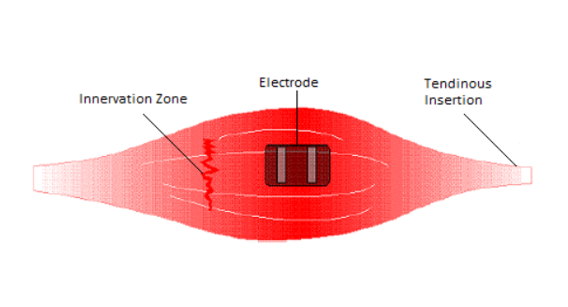
\includegraphics[scale=0.8]{imagenes/Disenodelsistema/electrodo.png}
	\caption{Posición de los electrodos}
	\label{fig:Posicion}
\end{figure}

\subsection{Obtención de señales}

Con lo visto en \ref{sec:Preparaciondelapiel} y \ref{sec:Loselectrodos} tendríamos que definir el músculo que va a hacer de instrumento de control para el sistema. Se plantea la idea de usar un músculo del antebrazo por la facilidad para la colocación de los electrodos, así como a la hora de descriminar los distintos movimientos que nos van a permitir el control del sistema. Un correcto sitio sería con los 2 electrodos en la parte central y el de referencia en el codo que es un punto con poca actividad eléctrica.\newline 

El \textit{músculo flexor del carpo} (figura \ref{fig:flexor}) será  el que eligiremos debido a su posición central, ya que permite contraerlo y relajarlo con facilidad. \newline Por lo tanto este será el músculo sobre el cual vamos a colocar los electrodos para realizar la toma de señales y empezar a discriminar los distintos movimientos. Las pruebas deberán hacerse para los dos brazos, ya que nos permitirá más grados de libertad a la hora de elegir el método de control del sistema.  

\begin{figure}[H]
	\center
	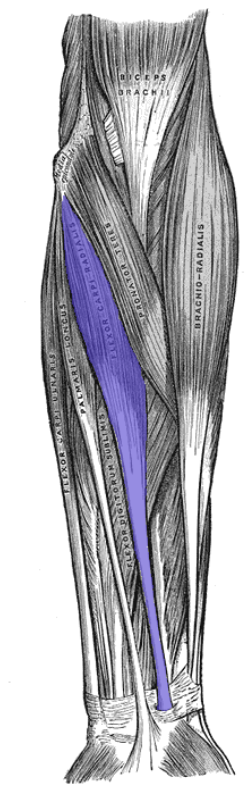
\includegraphics[scale=0.5]{imagenes/Disenodelsistema/flexor.png}
	\caption{Músculo flexor del carpo en el antebrazo}
	\label{fig:flexor}
\end{figure}


Se tomarán unas señales EMG de entrenamiento, que mediante Bluethooth son enviadas al ordenador en tiempo real y vistas en OpenSignals. En el mismo OpenSignals podemos seleccionar el intervalo de tiempo de la captación que queremos guardar, y nos ofrece distintos formatos para hacerlo: .edf .h5 y .txt. Entre ellos guardaremos las señales como un archivo de texto (.txt), que tendrán el número de muestra y su valor correspondiente.\newline 

Estos archivos .txt será lo que lea Matlab para realizar el procesamiento. \newline


\begin{figure}[H]
	\center
	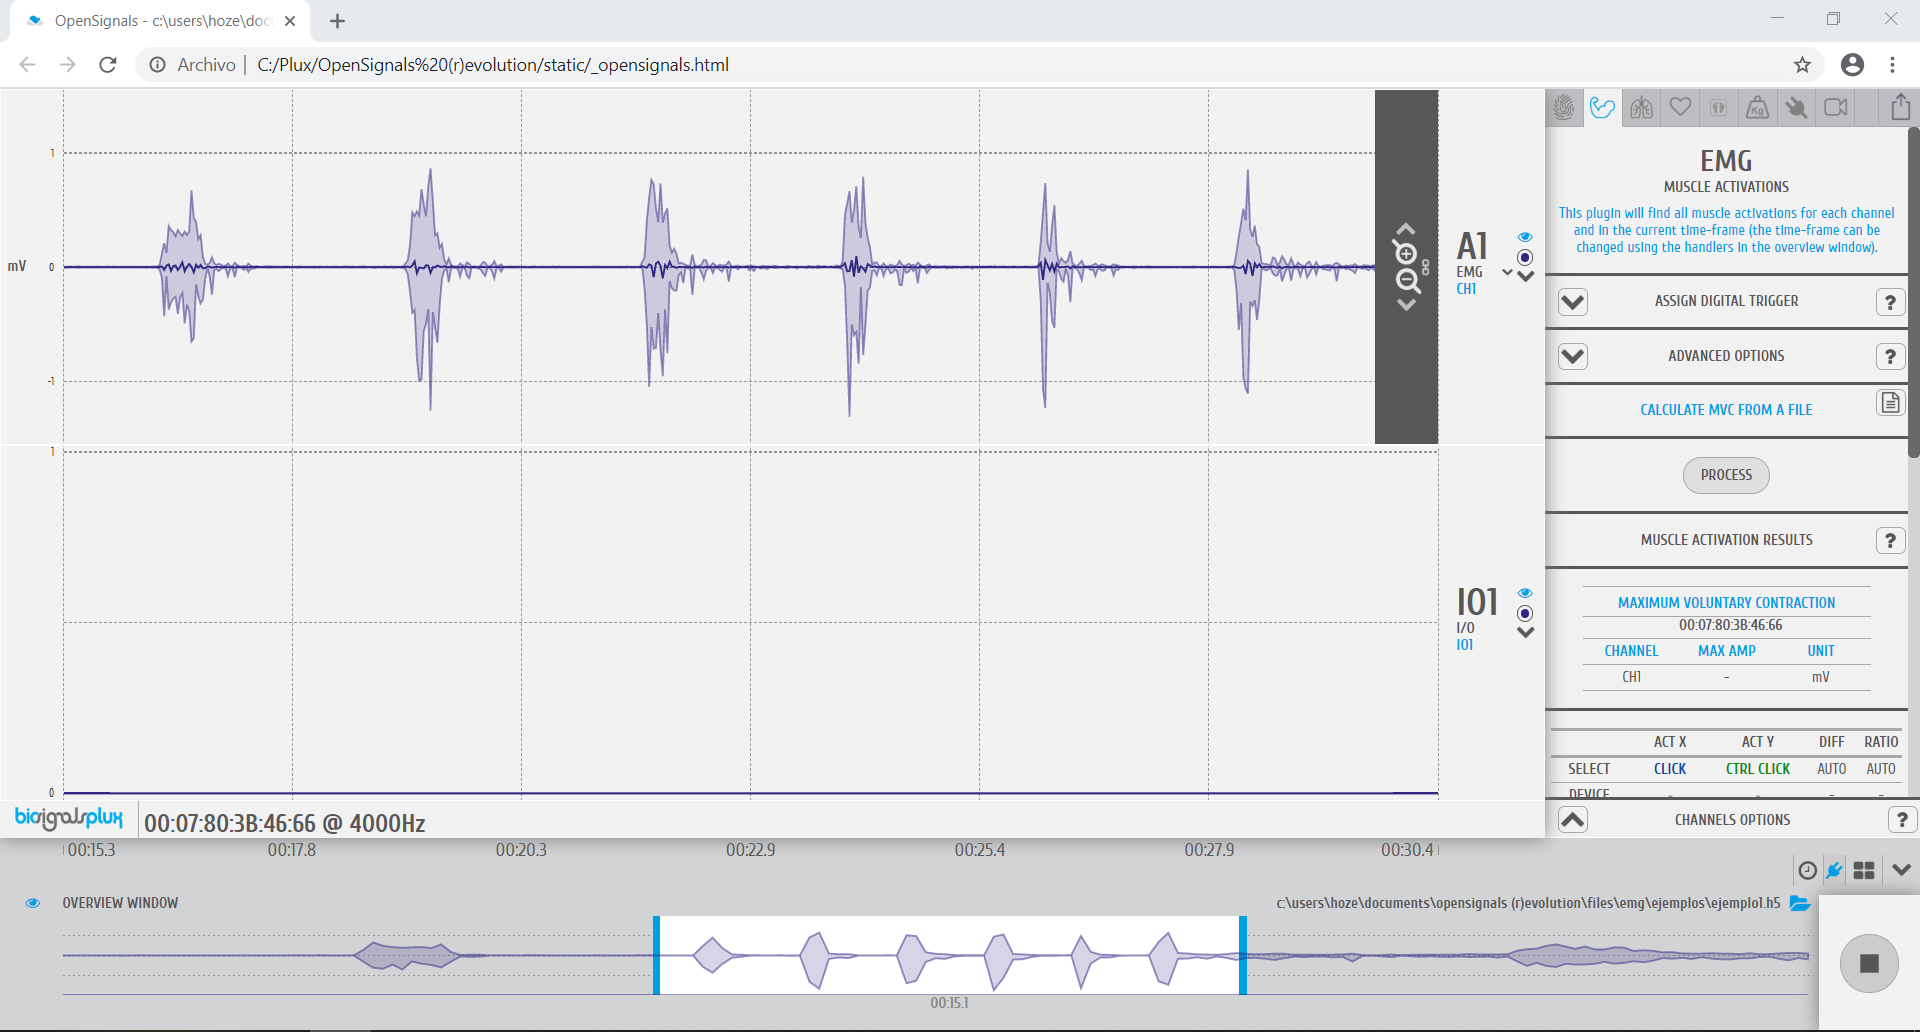
\includegraphics[scale=0.3]{imagenes/Disenodelsistema/ejemplo.png}
	\caption{Señal captada por OpenSignals}
	\label{fig:ejemplo}
\end{figure}



En la figura \ref{fig:ejemplo} se puede distinguir bastante bien las diferentes contracciones que ha sufrido el músculo en el proceso de obtención. Las zonas con una menor amplitud se tratan de relajaciones o momentos en los que el flexor se encuentra relajado y con poca actividad eléctrica. En el momento en el que contraemos voluntariamente el músculo se alcanzan picos de gran amplitud; que dependiendo de la fuerza de la contracción serán de mayor o menor intensidad. El algoritmo que creemos tendrá que ser carpaz por lo tanto de discriminar si el músculo se encuentra relajado o contraído.
Tras la obtención, un procesamiento con Matlab será necesario para acondicionarlas y preparar las señales para su uso.


\subsection{Procesamiento en Matlab}

A la hora de trabajar con bioseñales para el control de mecanismos robóticos, se necesitan señales sin interferencias. Las interferencias más comunes,como hemos visto en \ref{sec:Ruido} es el ruido de 50Hz de la red eléctrica; aunque también existen de otro tipo como las que ocurren en la medición, como el movimiento de los cables o incluso los problemas del mismo equipo que hace las medidas. \newline 

Para realizar el procesamiento digital de la señal EMG además será necesario tener en cuenta que la mayor parte de su información se encuentra en el rango de frencuencias de 5Hz a 500Hz. Debido a su comportamiento no determinista, debe procesarse con técnicas de caracterización que permitan conocer características definidas de la señal, a través de las cuales apicar los determinados métodos de control. \newline

Las señales en formato .txt son cargadas en Matlab mediante la función \textit{dlmread}, que lee los datos del fichero y los guarda en una matriz, donde el valor de la frecuencia de muestreo de la señal se almacena en una variable. Hay que tener en cuenta que los valores del fichero no son los valores reales de la señal, son valores muestreados que devuelve el programa; por lo que deben ser convertidos a voltaje usando una expresión matemática que nos facilita el manual de BioSignalplux.\newline

 La expresión matemática se define en \ref{eqn:ec1}:
\begin{equation}
EMG(V)=\frac{((ADC/2^n)-1/2)*Vcc}{G}
\label{eqn:ec1}
\end{equation}

Donde: 
\begin{itemize}
	\item Vcc= 3V (Voltaje de operación)
	\item G= 1000 (Ganancia del sensor)
	\item EMG(V) - Valor de la señal EMG en voltios
	\item ADC - Valor sampleado del canal que devuelve el programa
	\item n -Número de bits del canal
\end{itemize}


\begin{figure}[H]
	\center
	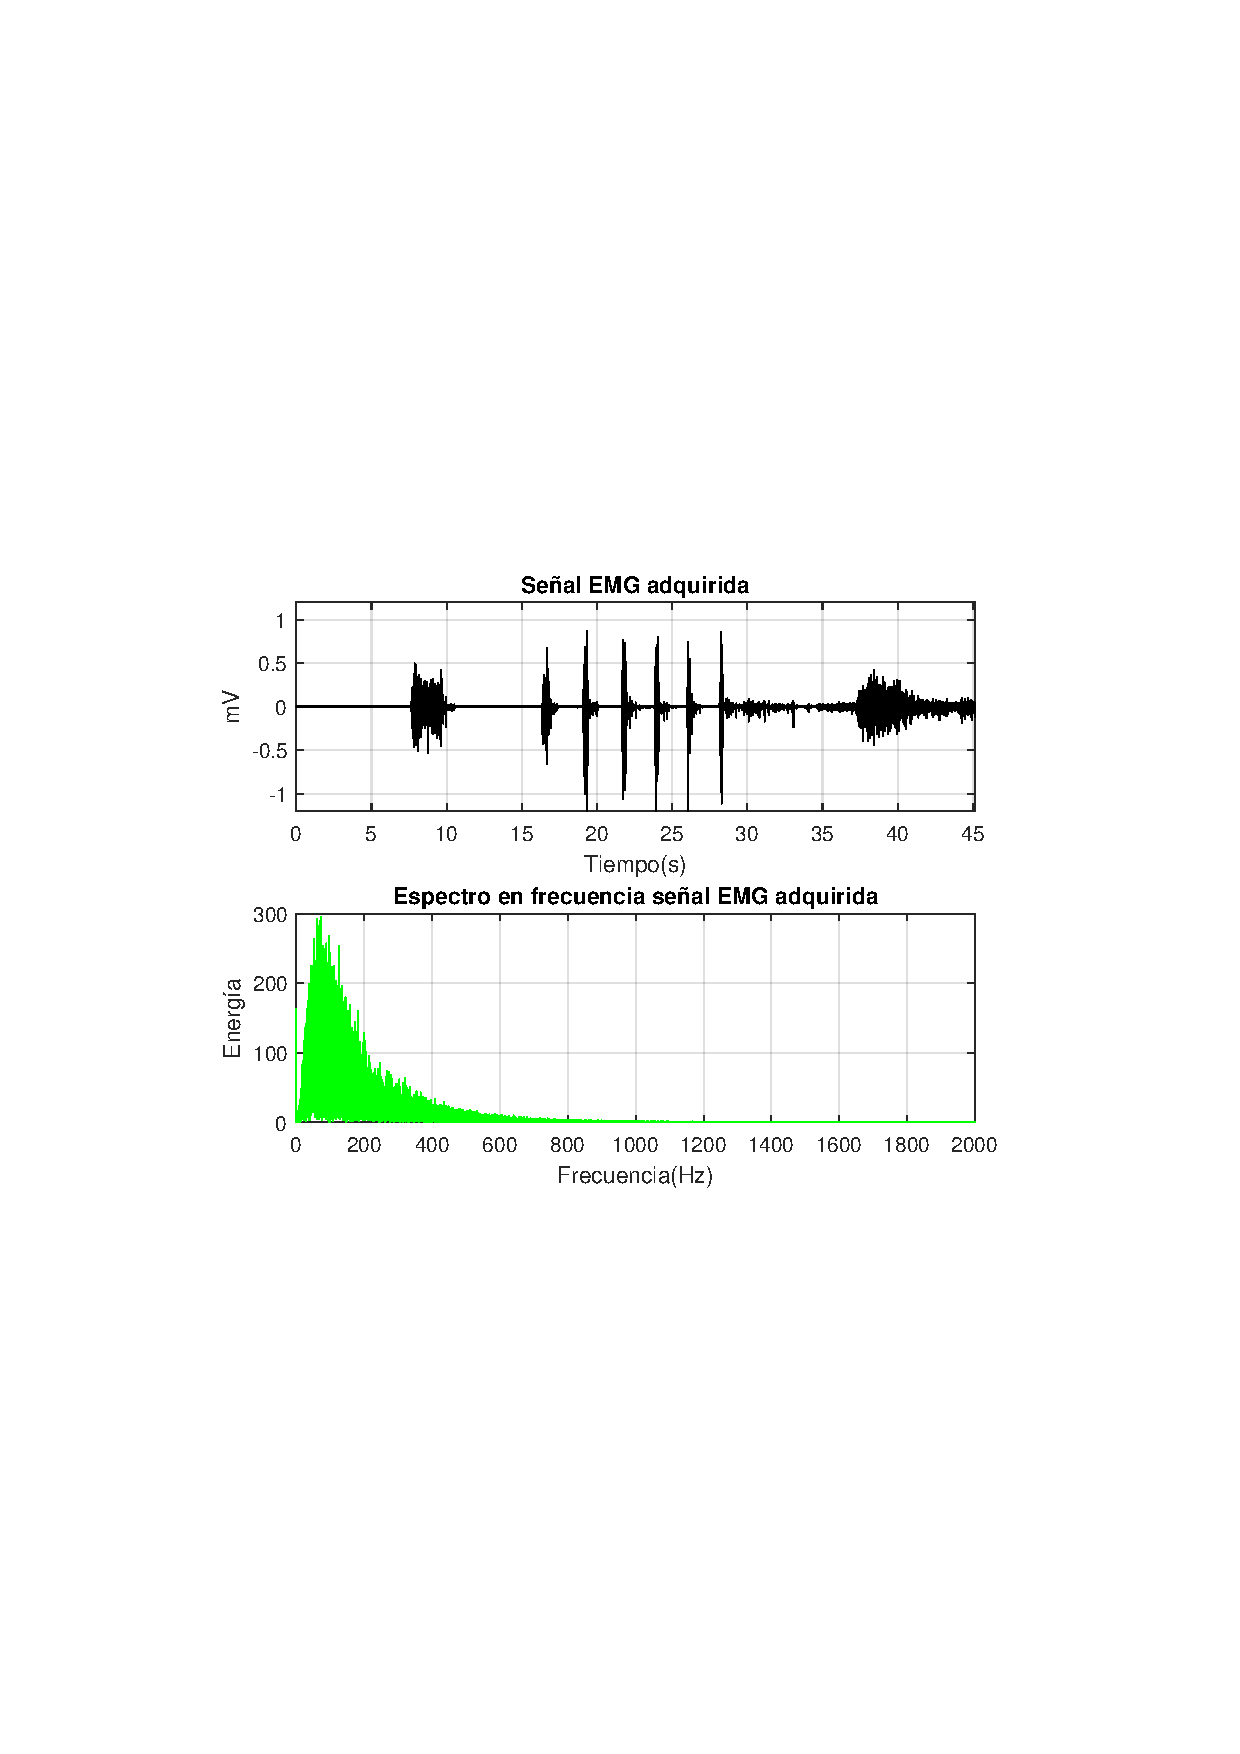
\includegraphics[scale=0.5]{imagenes/Disenodelsistema/graf1.png}
	\caption{Señal captada representada en Matlab}
	\label{fig:graf1}
\end{figure}

En la figura \ref{fig:graf1} se muestra la señal guardada una vez representada en Matlab en el dominio del tiempo y en el dominio de la frecuencia. Una vez tenemos la señal, si le hacemos la transformada rápida de fourier con el comando \textit{fft} podemos obtener su espectro correspondiente. Para que la señal sea óptima en las siguientes etapas será necesario filtrarla adecuadamente.

\subsubsection{Filtro de paso de banda EMG: 4Hz a 500Hz} \label{sec:pasobanda}

Como se ha comentado las señales EMG tiene su información más relevante en la banda de frecuencia entre 4Hz y 500Hz. Por esa razón, esto se toma como  criterio para el diseño de un filtro de paso banda, que puede ser entendido como un filtro pasa alto con frecuencia de corte de 4Hz en serie con un filtro paso bajo con frecuencias de corte de 500 Hz. \newline
Se elige que este filtro sea de Butterworth, ya que permite la respuesta más plana posible. Su función de transferencia es la siguiente:

\begin{equation}
|H(w)|^2 = \frac{1}{1+(w/wc)^(2N)}
\end{equation}

Donde: 
\begin{itemize}
	\item N es el orden del filtro
	\item wc es la frecuencia de corte 
	\item w la frecuencia compleja 
\end{itemize}

El filtro  de manera matemática puede ser complejo de calcular, pero Matlab cuenta con la función \textit{butter}  que lo hace automáticamente; especificando las frecuencias de corte y el orden del filtro. 
\begin{figure}[H]
	\center
	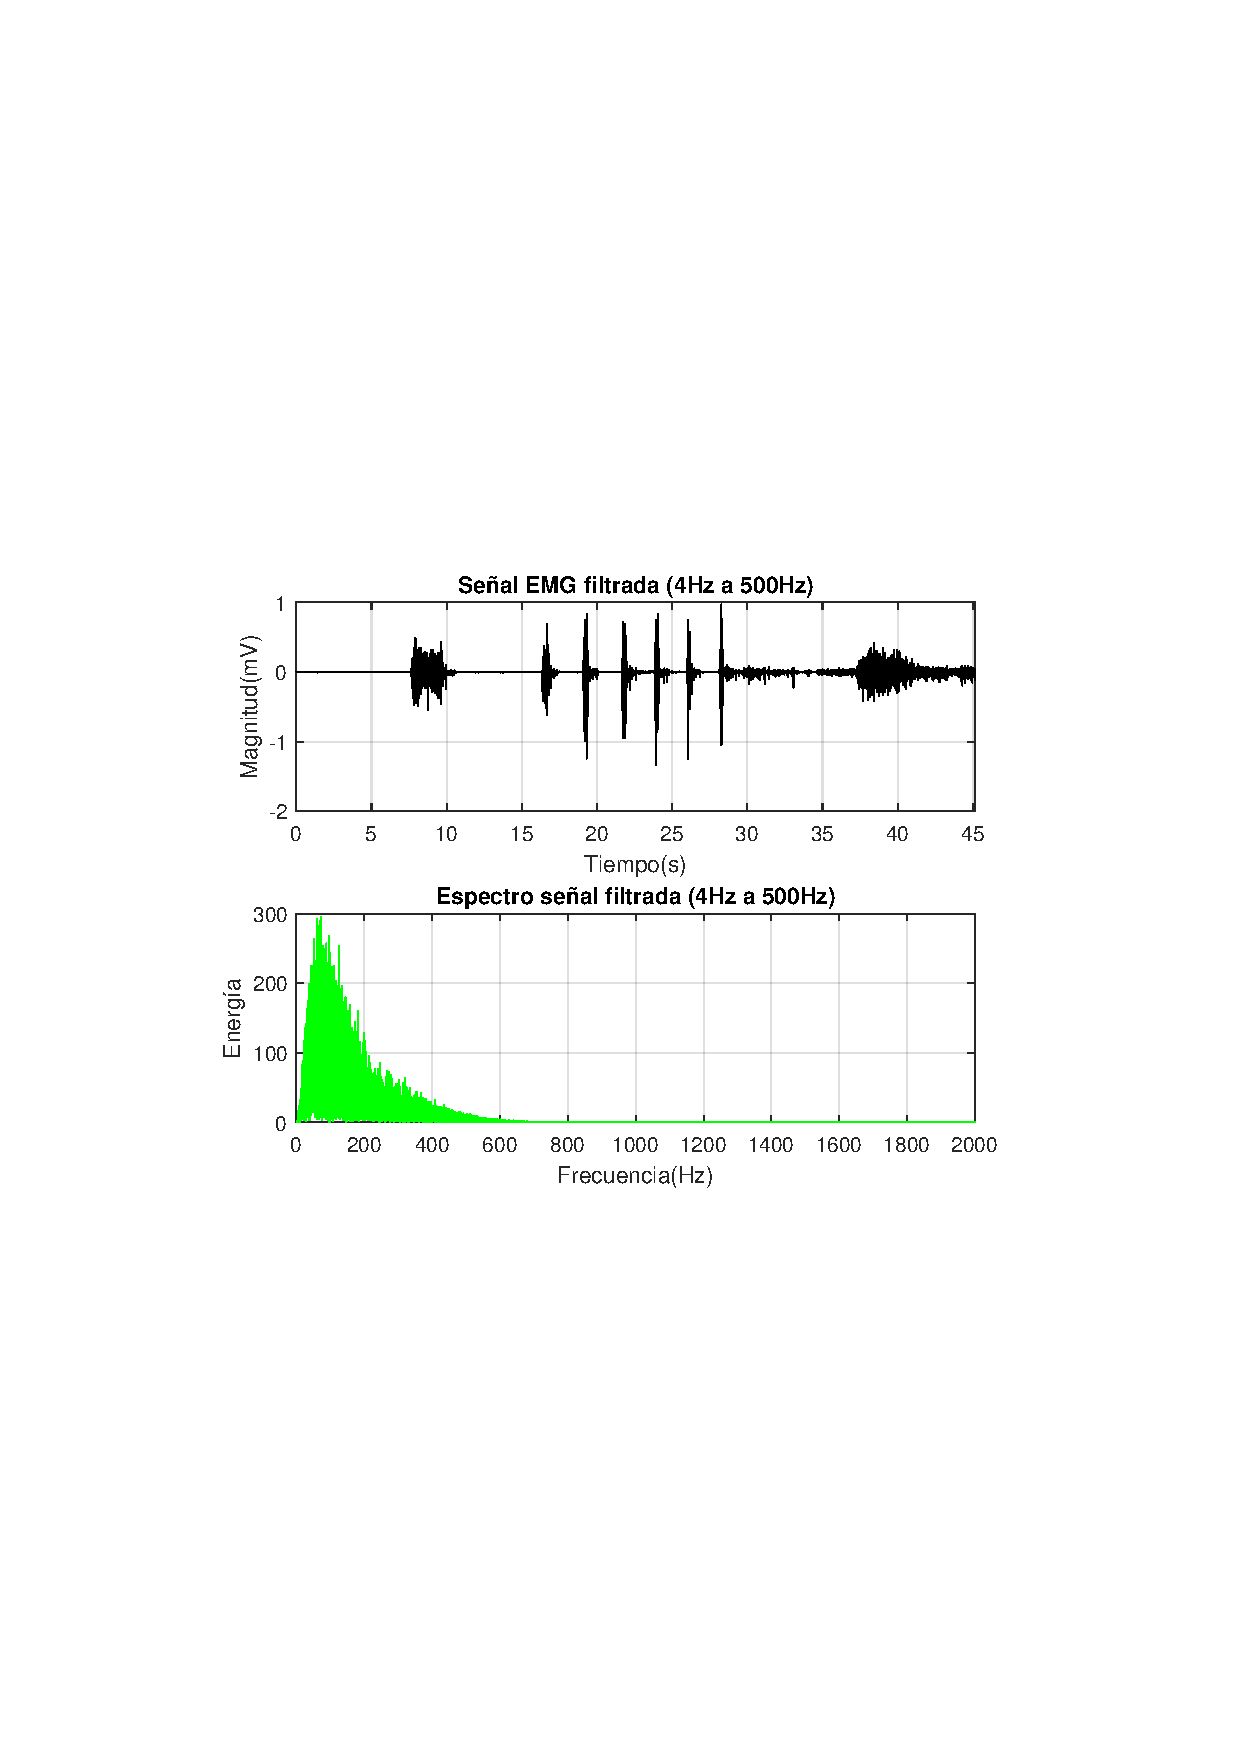
\includegraphics[scale=0.5]{imagenes/Disenodelsistema/graf2.png}
	\caption{Señal con el filtro paso banda}
	\label{fig:graf2}
\end{figure}

En la figura \ref{fig:graf2} la señal ya quedaría con la información más relevante en la banda 4Hz-500Hz, desechando las altas frecuencias que interfieran en la señal. 

\subsubsection{Filtro de rechazo banda EMG: 50Hz}

En España, la frecuencia de la línea eléctrica es de 50Hz, por lo que se requiere el diseño de un filtro rechazo banda que elimine este ruido. Se lleva a cabo el mismo procedimiento que en \ref{sec:pasobanda} para el diseño de un filtro de rechazo banda de 50Hz. Para ello se usa de nuevo la función \textit{butter} pero esta vez con el parámetro \textit{stop} para que sea de rechazo. Esta nueva filtración se añade a la anterior, dejando las señales libres de ruido y acondicionadas para sacar sus parámetros de bondad.

\begin{figure}[H]
	\center
	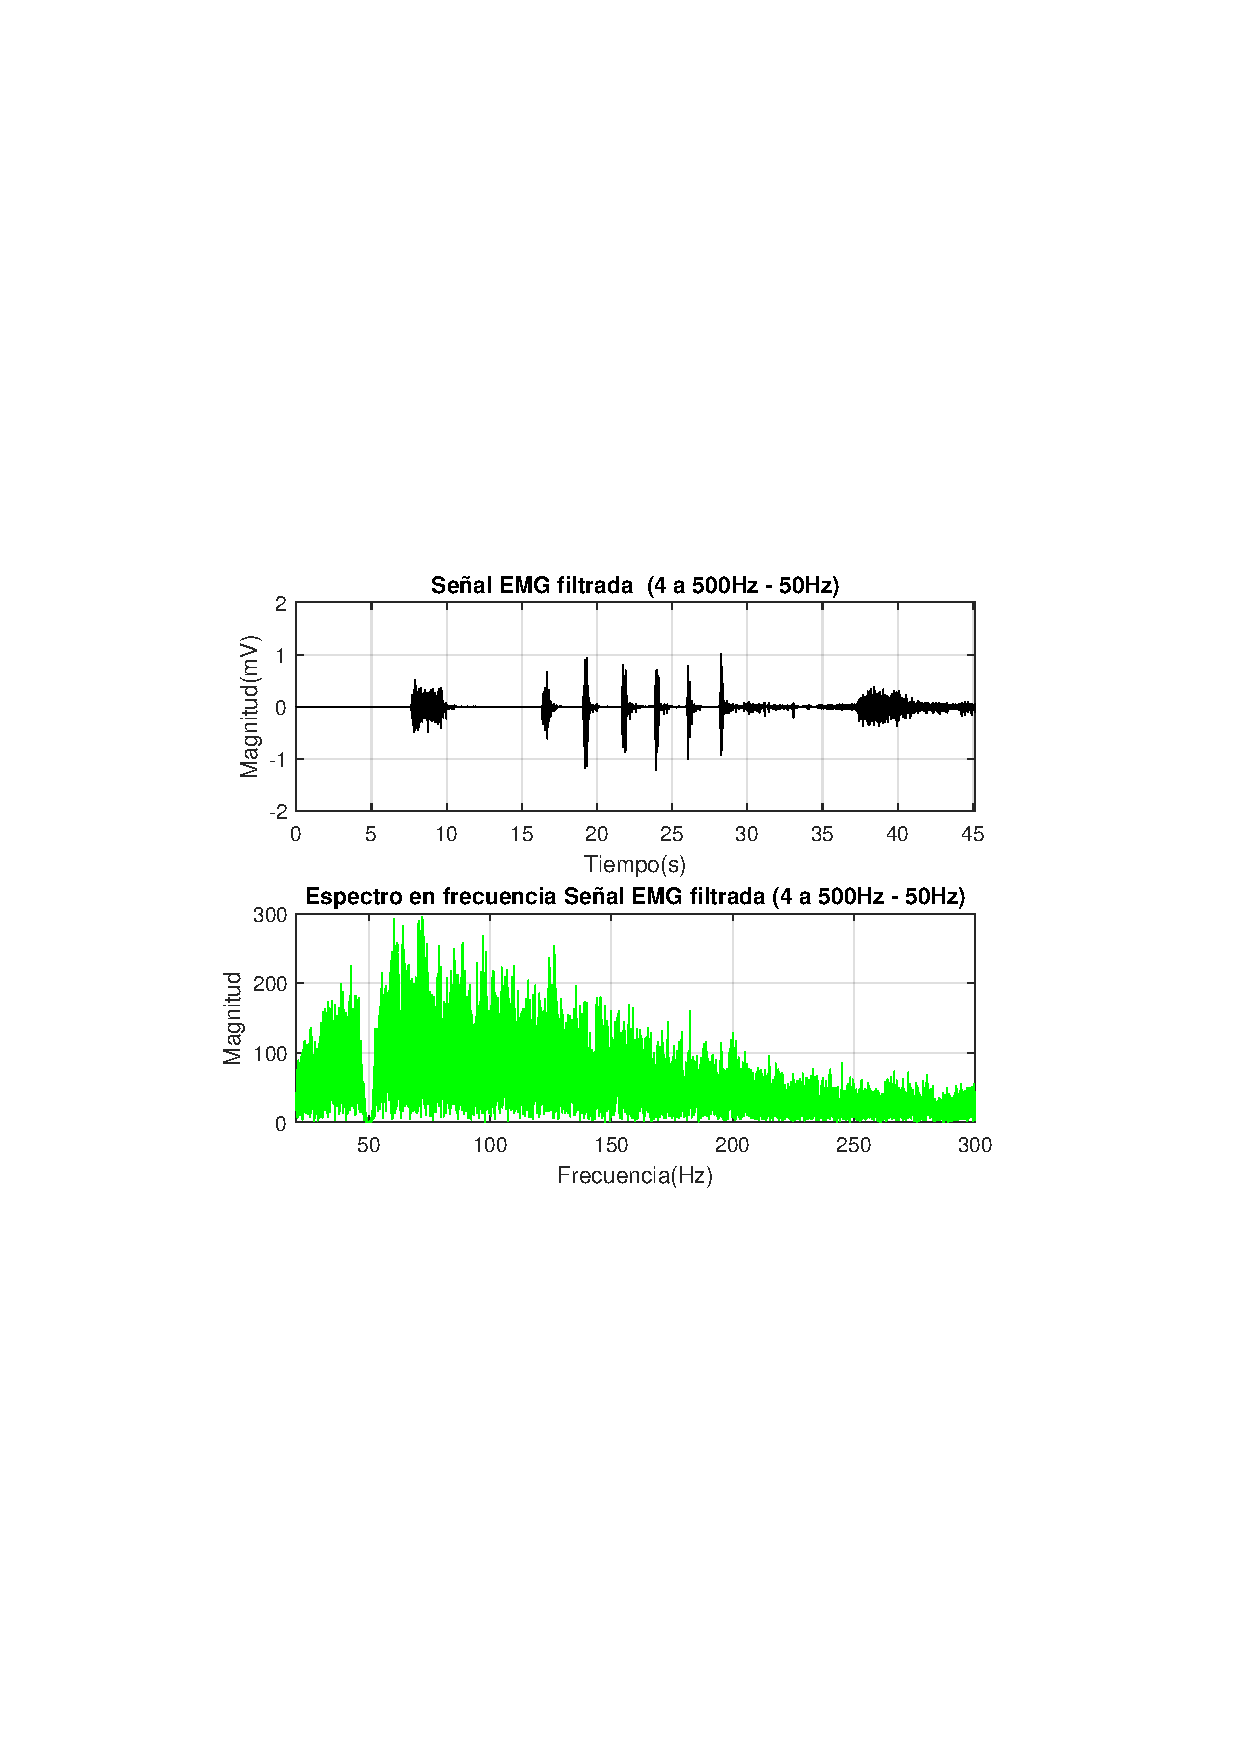
\includegraphics[scale=0.5]{imagenes/Disenodelsistema/graf3.png}
	\caption{Señal con el filtro paso banda y el rechazo banda}
	\label{fig:graf3}
\end{figure}

Haciendo la comparación de la señal antes y después del filtrado, se puede ver el resultado de los filtros. En la figura \ref{fig:graf4} se representa en rojo la señal original y en negro la señal una vez acondicionada. 

\begin{figure}[H]
	\center
	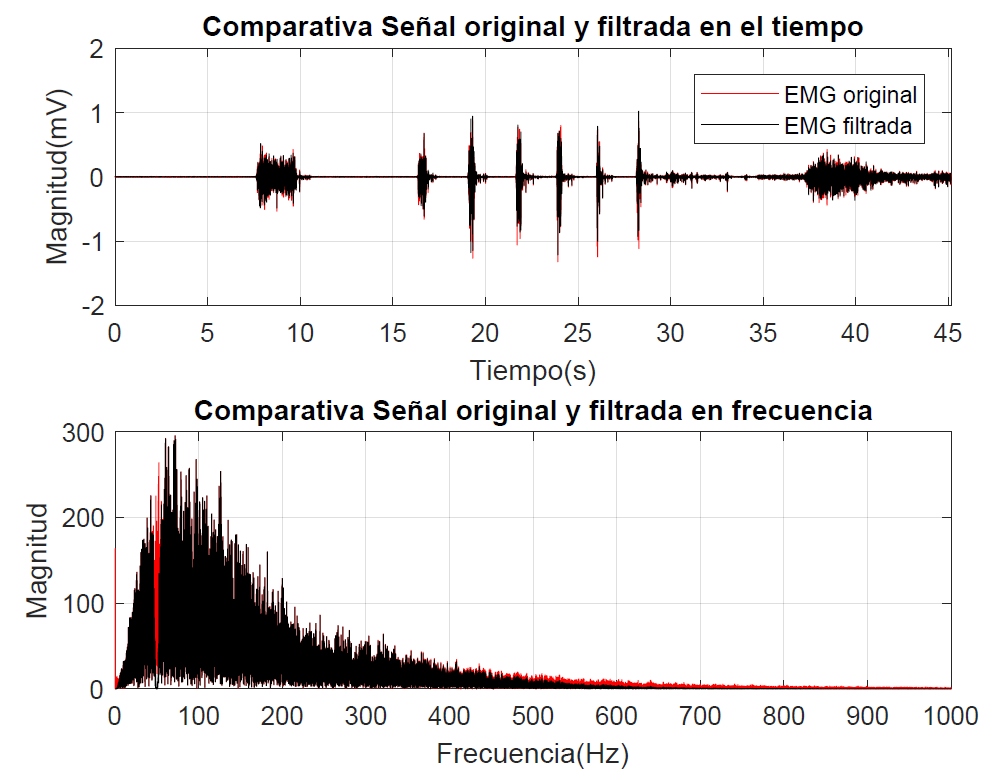
\includegraphics[scale=0.5]{imagenes/Disenodelsistema/graf4.png}
	\caption{Comparativa antes y después del los filtros}
	\label{fig:graf4}
\end{figure}

\subsubsection{Caracterización de la señal}

Una vez la señal está acondicionada adecuadamente, se implementan técnicas de caracterización para sacar parámetros que nos permitan reconocer los distintos movimientos. Se necesitan herramientas para obtener la energía promedio de la señal que nos permitan caracterizar los distintos cambios que sufre esta dependiendo de la contracción.
La señal EMG es muy oscilante (puede cambiar rápidamente en un milisegundo) por lo que resultaría imposible utilizarla directamente para controlar un sistema robótico. Se necesita un método que permita obtener características de la señal y poder definir patrones o comportamientos de ésta. \newline

Una manera de caracterizar una señal es usando el \textit{método por ventanas} que calcula la envolvente de la señal EMG. Para ello dividimos la señal en segmentos o ventanas de longitud L de 250ms con un solapamiento entre ventanas de 125ms, y caracterizamos usando la \textit{Suma de valores absolutos} o \textit{IAV}. Cuanto menor sea L y más alto el solapamiento, mayor número de ventanas y mejor caracterización; pero el procesamiento será más lento. \newline

La IAV \textit{suma de valores absolutos} realiza la suma de los valores absolutos contenidos en cada una de las secciones o ventanas en las que hemos dividido la señal, para dar una idea aproximada de la intensidad de esa ventana. \newline


 La expresión de la IAV se define en \ref{eqn:ec2}:

\begin{equation}
EMG_IAV=\sum_{k=1}^{N}|EMG_{k}|, i=0,......,L-1.
\label{eqn:ec2}
\end{equation}

Esto nos permite distinguir mediante umbrales los grados de intensidad de la señal obtenida, cuanto más tensión se aplique más energía tendrá la señal EMG, lo que se traducirá en un pico más grande de la IAV.
Con esto ya podemos decir que si una señal pasa determinado umbral será una contracción fuerte, contracción leve o relajación.

\begin{figure}[H]
	\center
	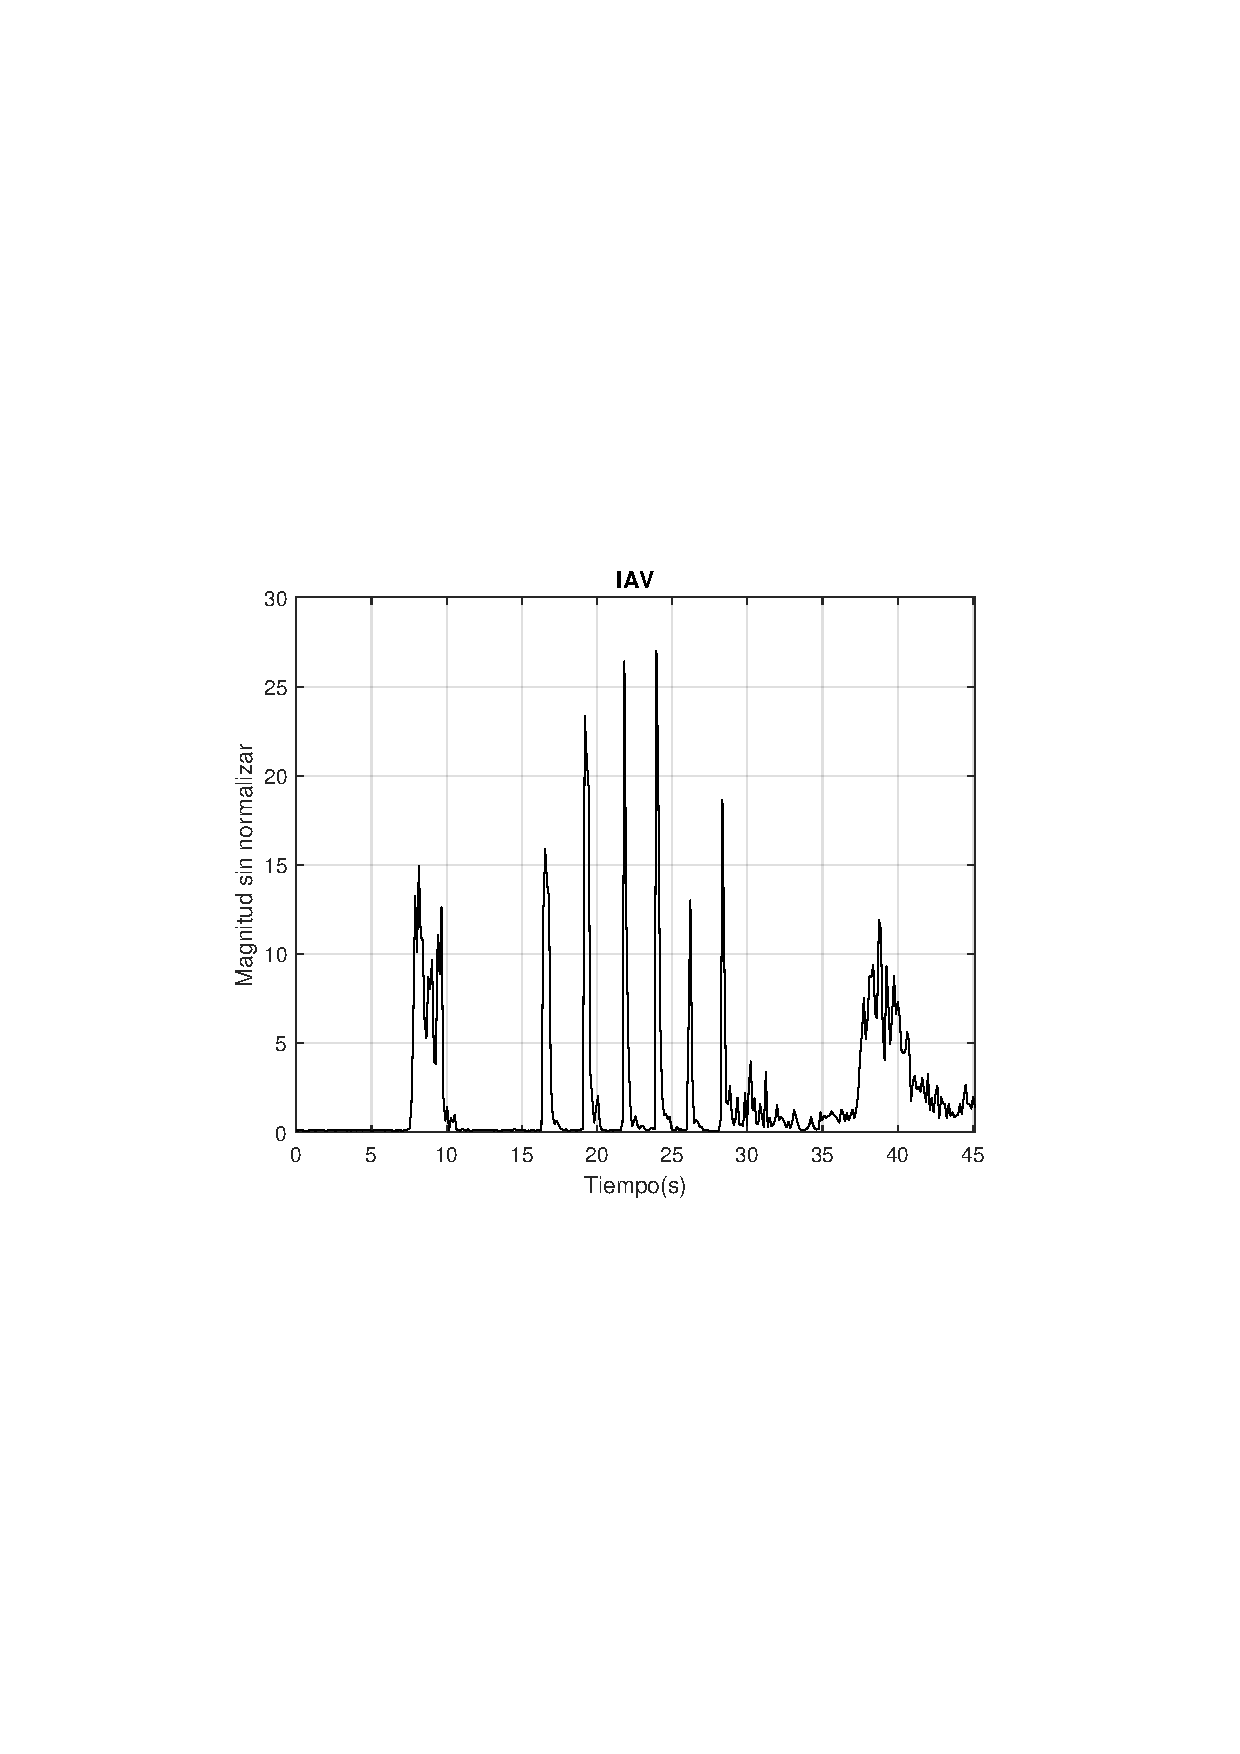
\includegraphics[scale=0.5]{imagenes/Disenodelsistema/graf5.png}
	\caption{Representación de la IAV}
	\label{fig:graf5}
\end{figure}

\subsubsection{Testeo del algoritmo}

Para el testeo del algoritmo se propone usar varias señales tomadas posteriormente,sin modificar el algoritmo de procesamiento. Para ello recogemos una serie de señales de pruebas, en concreto 10 con el brazo derecho y 10 con el brazo izquierdo. Se ha tratado de realizar en todos las señales captadas los mismos movimientos a diferentes velocidades y orden, para ver si el algoritmo es capaz de distinguirlos correctamente.  \newline

En principio nos interesa poder identificar en las señales tres movimientos con cada brazo, que tendrán distintos niveles de tensión para el músculo.

	\begin{itemize}
	\item \textbf{El músculo relajado.} En el que la contracción, y por lo tanto la IAV será mínima.
	\item \textbf{El músculo contraído levemente.} La IAV presentará mayor amplitud.
	\item \textbf{El músculo contraído y con el brazo girado.} La contracción será máxima y mucho mayor la IAV que en los otros dos movimientos.
	\end{itemize}

En la tabla \ref{tabla:tabla1} recogemos las pruebas hechas con el algoritmo para las diferentes señales captadas con cada brazo. El algoritmo es capaz de procesar y discriminar cada señal correctamente. 

\renewcommand\tablename{Tabla}
\begin{table}[H]
\centering
\begin{tabular}{|l|l|l|l|l|}
\hline
\multicolumn{2}{|l|}{}                       & Relajación & Contracción & Giro \\ \hline
\multirow{10}{*}{Brazo derecho}   & Señal 1  & OK         & OK          & OK   \\ \cline{2-5} 
                                  & Señal 2  & OK         & OK          & OK   \\ \cline{2-5} 
                                  & Señal 3  & OK         & OK          & OK   \\ \cline{2-5} 
                                  & Señal 4  & OK         & OK          & OK   \\ \cline{2-5} 
                                  & Señal 5  & OK         & OK          & OK   \\ \cline{2-5} 
                                  & Señal 6  & OK         & OK          & OK   \\ \cline{2-5} 
                                  & Señal 7  & OK         & OK          & OK   \\ \cline{2-5} 
                                  & Señal 8  & OK         & OK          & OK   \\ \cline{2-5} 
                                  & Señal 9  & OK         & OK          & OK   \\ \cline{2-5} 
                                  & Señal 10 & OK         & OK          & OK   \\ \hline
\multirow{10}{*}{Brazo izquierdo} & Señal 1  & OK         & OK          & OK   \\ \cline{2-5} 
                                  & Señal 2  & OK         & OK          & OK   \\ \cline{2-5} 
                                  & Señal 3  & OK         & OK          & OK   \\ \cline{2-5} 
                                  & Señal 4  & OK         & OK          & OK   \\ \cline{2-5} 
                                  & Señal5   & OK         & OK          & OK   \\ \cline{2-5} 
                                  & Señal 6  & OK         & OK          & OK   \\ \cline{2-5} 
                                  & Señal 7  & OK         & OK          & OK   \\ \cline{2-5} 
                                  & Señal 8  & OK         & OK          & OK   \\ \cline{2-5} 
                                  & Señal 9  & OK         & OK          & OK   \\ \cline{2-5} 
                                  & Señal 10 & OK         & OK          & OK   \\ \hline
\end{tabular}
	\caption{Señales de prueba y resultados}
	\label{tabla:tabla1}
\end{table}
\newpage

\subsection{Comunicación serie en Matlab}

Una vez procesadas las señales tenemos que pasarlas a la FPGA para el diseño del sistema de control. El \textit{puerto serie} nos abre la posibilidad de comunicar el ordenador con nuestros circuitos en la FPGA, y por lo tanto poder enviar datos de x bits. Se trata de comunicaciones serie asíncronas y se utiliza un único cable de datos para recepción y transmisión. Tras la clasificación de las señales con la IAV ajustamos el rango de datos obtenido de 0 a 255  (8bits) en Matlab y estos se envían mediante el puerto serie (COM7) a la FPGA.\newline

Para ello será necesario abrir el puerto serie del ordenador con el comando \textit{fopen}, enviar los datos con \textit{fwrite} y definir la velocidad de transmisión, que será para toda la transmisión y recepción de 115200 baudios.

\section{Diseño en icestudio}

\subsection{Receptor serie}\label{sec:rserie}

La FPGA icezum Alhambra que vamos a utilizar ofrece a través del USB una interfaz de comunicaciones serie síncronas (por la que se realiza la carga del programa creado en Icestudio a la placa) y una interfaz de puerto serie. Por lo tanto para realizar la conexión entre PC-FPGA bastaría con conectarlos mediante un USB para tener listo el hardware de envío de datos. No solo es necesario abrir el puerto serie por Matlab, también la FPGA necesita para recibirlos un receptor serie, que habrá que crearlo en Icestudio.\newline

El esquema del receptor de bits mediante el puerto serie planteado se muestra en la figura \ref{fig:receptorserie}:

\begin{figure}[H]
	\center
	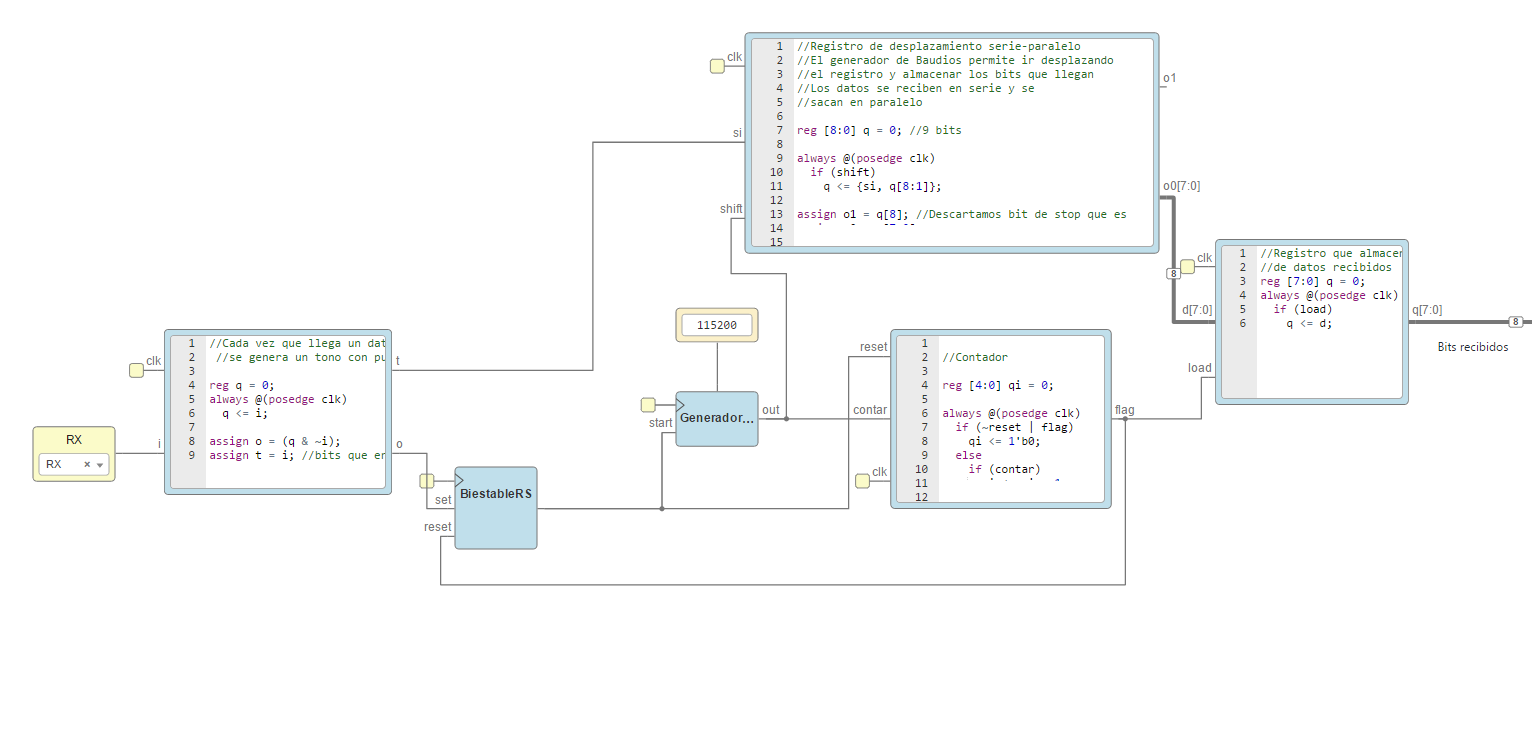
\includegraphics[scale=0.5]{imagenes/Disenodelsistema/receptorserie.png}
	\caption{Receptor serie en icestudio}
	\label{fig:receptorserie}
\end{figure}

Los bits deben de llegar por el puerto serie y salir por un bus de 8 bits  en paralelo para poder utilizar los datos que llegan. 
\begin{figure}[H]
	\center
	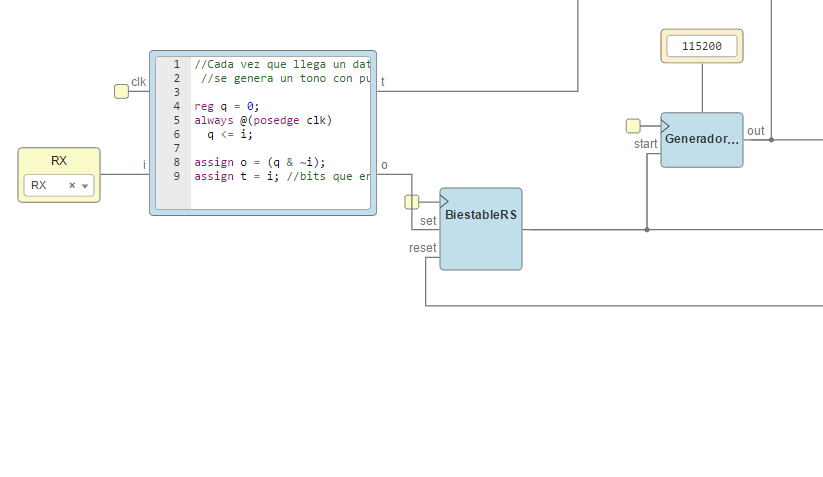
\includegraphics[scale=0.7]{imagenes/Disenodelsistema/receptorserie1.png}
	\caption{Primera parte del receptor serie}
	\label{fig:receptorserie1}
\end{figure}

Por RX llegan los bits en tramas en serie, primero el bit de start, después los bits empezando por el menos significativo y luego el bit de stop. Cada vez que llega un bit de start (que una trama es enviada) se genera un tono puro que activa un biestable RS; el cuál se reseteará para recibir un nuevo dato. Éste a su vez activa un generador de baudios a la velocidad de recepción serie de 115200 baudios.\newline
\begin{figure}[H]
	\center
	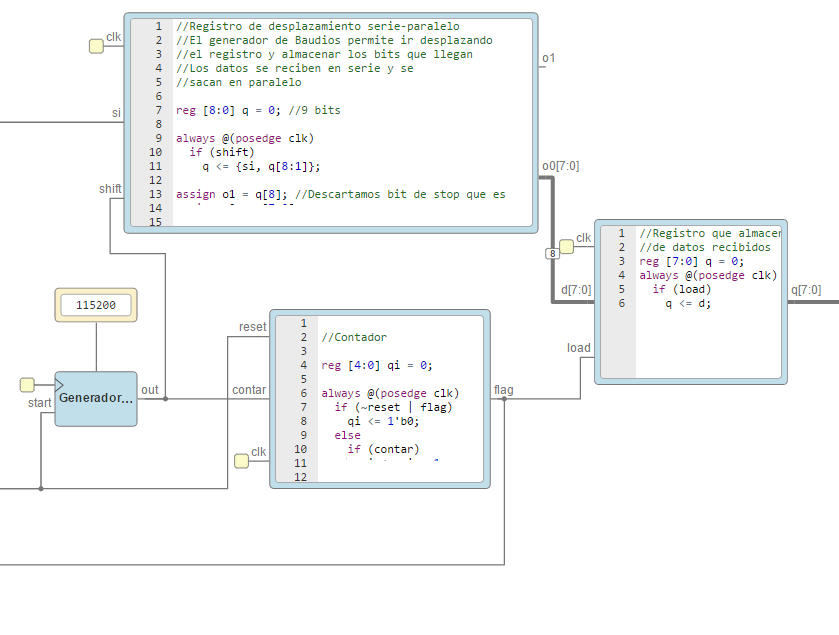
\includegraphics[scale=0.7]{imagenes/Disenodelsistema/receptorserie2.png}
	\caption{Segunda parte del receptor serie}
	\label{fig:receptorserie2}
\end{figure}


Con el generador de baudios se generan los tics para leer los bits serie que van llegando a una velocidad determinada. La salida del generador va a un registro de desplazamiento serie-paralelo y a un contador.El generador de Baudios permite ir desplazando el registro y almacenar los bits que llegan.Los datos se reciben en serie y se sacan en paralelo.A su vez que el generador de baudios genera un tic se incrementa el contador. Al llegar a 9 bits ( 8 datos y 1 stop- el de start solo es para arrancar) significa que ya ha llegado el dato completo y se  activa el flag que reinica el biestable RS y se queda listo para recibir un nuevo dato.
\subsection{Modulador de PWM}

Como hemos visto en \ref{sec:comdron} el dron necesita recibir las señales mediante un protocolo de comunicaciones. Por lo tanto habrá que adaptar las señales recibidas en la FPGA a una modulación PWM. \newline

La Modulación por anchura de pulsos nos va a permitir generar señales analógicas a partir de sistemas digitales.  Esto se puede usar por ejemplo para mover un motor a diferentes velocidades, o cambiar la intensidad con la que brilla un led. Para nuestra aplicación nos va a permitir enviarle las órdenes al dron, y definir un sistema de control en base a las señales que hemos obtenido con el receptor serie. \ref{sec:rserie}

Para ello se ha creado el bloque PWM de la figura \ref{fig:bloquepwm}

\begin{figure}[H]
	\center
	\includegraphics[scale=0.7]{imagenes/Disenodelsistema/bloquePWM.png}
	\caption{Bloque PWM}
	\label{fig:bloquepwm}
\end{figure}

Para cada entrada de datos de 8 bits se genera una señal de PWM en la salida. La estructura del bloquePWM es la siguiente:

\begin{figure}[H]
	\center
	\includegraphics[scale=0.5]{imagenes/Disenodelsistema/bloquePWM2.png}
	\caption{Estructura del Bloque PWM}
	\label{fig:bloquepwm2}
\end{figure}

Ésta cuenta con 2 elementos principales:

	\begin{itemize}
	\item \textbf{Un contador de reloj.} El contador tiene N bits. N va a determinar la frecuencia y tendremos que elegirla por lo tanto antes de el diseño del contador
	\item \textbf{Un registro de anchura.} El valor de anchura de pulso será el dato que llega por la entrada; es la información que se recibe del sistema de adquisición.
	\end{itemize}

La frecuencia que tenga la señal PWM por lo tanto, podremos obtenerla a partir de la señal de reloj del sistema de 12 MHz con un divisor de frecuencia. Para ello tenemos que tener en cuenta la frecuencia que deseemos, que se presentan en la tabla \ref{tabla:tabla2}.

\begin{table}[H]
\centering
\begin{tabular}{lll}
\hline
 \multicolumn{1}{|l|}{Frecuencia} & \multicolumn{1}{l|}{Reloj(S)}                      \\ \hline
 \multicolumn{1}{|l|}{12 MHZ}     & \multicolumn{1}{l|}{S}                             \\ \hline
 \multicolumn{1}{|l|}{6 MHZ}      & \multicolumn{1}{l|}{S/2}                           \\ \hline
 \multicolumn{1}{|l|}{3 MHZ}      & \multicolumn{1}{l|}{S/4}                           \\ \hline
 \multicolumn{1}{|l|}{1.5 MHZ}    & \multicolumn{1}{l|}{S/8}                           \\ \hline
 \multicolumn{1}{|l|}{750 KHZ}    & \multicolumn{1}{l|}{S/16}                          \\ \hline
 \multicolumn{1}{|l|}{375 KHZ}    & \multicolumn{1}{l|}{S/32}                          \\ \hline
 \multicolumn{1}{|l|}{187.5 KHZ}  & \multicolumn{1}{l|}{S/64}                          \\ \hline
 \multicolumn{1}{|l|}{93.8 KHZ}   & \multicolumn{1}{l|}{S/128}                         \\ \hline
 \multicolumn{1}{|l|}{46.9 KHZ}   & \multicolumn{1}{l|}{S/256}                         \\ \hline
 \multicolumn{1}{|l|}{23.4 KHZ}   & \multicolumn{1}{l|}{S/512} \\ \hline
 \multicolumn{1}{|l|}{11.7 KHZ}   & \multicolumn{1}{l|}{S/1024}    \\ \hline
 \multicolumn{1}{|l|}{5.9 KHZ}    & \multicolumn{1}{l|}{S/2048}                        \\ \hline
 \multicolumn{1}{|l|}{2.9 KHZ}    & \multicolumn{1}{l|}{S/4096}                        \\ \hline
 \multicolumn{1}{|l|}{1.5 KHZ}    & \multicolumn{1}{l|}{S/8192}                        \\ \hline
 \multicolumn{1}{|l|}{732 Hz}     & \multicolumn{1}{l|}{S/16384}                       \\ \hline
 \multicolumn{1}{|l|}{366 Hz}     & \multicolumn{1}{l|}{S/32768}                       \\ \hline
 \multicolumn{1}{|l|}{183 Hz}     & \multicolumn{1}{l|}{S/65536}                       \\ \hline
 \multicolumn{1}{|l|}{92 Hz}      & \multicolumn{1}{l|}{S/131072}                      \\ \hline                                                  
\end{tabular}
	\caption{Frecuencias y Reloj del sistema}
	\label{tabla:tabla2}
\end{table}

Si queremos por ejemplo una señal PWM de 92 Hz, tenemos que usar un contador de 17 bits \ref{eqn:reloj}. Esta corresponde a un periodo de 11ms aproximadamente, que será el que usemos para nuesta aplicación.

\begin{equation}
Bits(N)= \frac{Reloj del sistema(12Mhz)} {131072}=17 bits.
\label{eqn:reloj}
\end{equation}

En el divisor de frecuencias los 8 bits más significativos se extraen y estos se comparan con los 8 bits que llegan del registro de anchura W. Esta comparación es lo que permite generar los ciclos de PWM.

	\begin{itemize}
	\item Si el contador es \textbf{menor} que el registro de anchura. La salida será 1.
	\item Si contador es \textbf{mayor} que el registro de anchura . La salida será 0.
	\end{itemize}